\section{多元变换}
\label{sec:rvt-multivariate}

随机向量$\bm{X}=(X_1,\ldots,X_d)$有联合密度$f_{\bm{X}}$，$\bm{Y}=\bm{g}(\bm{X})$取值于$\mathbb{R}^{k}$。原像规则~\eqref{eq:rvt-preimage-rule}仍然成立，难处在于原像是$\mathbb{R}^{d}$中的区域，把它的积分换到$\bm{Y}$的坐标上，要先回答三个问题：输入输出的维数是否相同，$\bm{g}$是否一一，是否需要像上一节那样分支。

\paragraph{仿射变换的均值与协方差}
先看最简单的$\bm{Y}=\bm{A}\bm{X}+\bm{b}$，其中$\bm{A}\in\mathbb{R}^{k\times d}$是确定的矩阵，$\bm{b}\in\mathbb{R}^{k}$。设$\bm{X}$有均值向量$\bm{\mu}$与协方差矩阵$\bm{\Sigma}$。由期望的线性性，
\[
 \mathbb{E}[\bm{Y}]=\bm{A}\bm{\mu}+\bm{b} .
\]
中心化之后$\bm{Y}-\mathbb{E}[\bm{Y}]=\bm{A}(\bm{X}-\bm{\mu})$，矩阵$\bm{A}$可以移到期望之外，于是
\begin{equation}
 \operatorname{Cov}(\bm{Y})=\mathbb{E}\bigl[\bm{A}(\bm{X}-\bm{\mu})(\bm{X}-\bm{\mu})^{\top}\bm{A}^{\top}\bigr]=\bm{A}\bm{\Sigma}\bm{A}^{\top} .
 \label{eq:rvt-affine-covariance}
\end{equation}
这两个公式对任何有有限二阶矩的$\bm{X}$都成立，不需要密度。

支撑也跟着变：$\bm{Y}$只在$\bm{X}$的取值范围在仿射映射下的像中取值。$k=d$而$\bm{A}$奇异时，像落在一个低维的仿射子空间里。例如
\[
 \bm{A}=\begin{pmatrix}1&1\\1&1\end{pmatrix},\qquad Y_1=Y_2=X_1+X_2 ,
\]
$\bm{Y}$总在对角线上。对角线在平面上面积为零，$\bm{Y}$没有二维的联合密度；由式~\eqref{eq:rvt-affine-covariance}，$X_1,X_2$独立且方差为$1$时$\operatorname{Cov}(\bm{Y})$的四个元素都是$2$，这个矩阵奇异，与支撑的退化相对应。所以求密度之前要先检查维数与可逆性。

\subsection{可逆变换}
\label{sec:rvt-invertible}

同维且一一的映射是一元单调变换的直接推广。一元时长度伸缩$\lvert g'\rvert$倍；多元时把小区间换成小方块，伸缩的是体积。

\paragraph{体积的伸缩}
可微映射在一点附近近似于线性映射$\bm{x}\mapsto\bm{g}(\bm{x}_0)+D\bm{g}(\bm{x}_0)(\bm{x}-\bm{x}_0)$，其中$D\bm{g}$是Jacobian矩阵。线性映射把任何区域的体积乘以行列式的绝对值，所以边长$\Delta$的小方块被映成体积约为$\lvert\det D\bm{g}(\bm{x}_0)\rvert\Delta^{d}$的小平行体。概率不变而体积放大$\lvert\det D\bm{g}\rvert$倍，密度就要除以这个数。

\begin{theorem}[可逆变换的联合密度]
\label{thm:rvt-multivariate-density}
设$\bm{X}$的联合密度在开集$U\subset\mathbb{R}^{d}$之外为零，$\bm{g}:U\to V=\bm{g}(U)$是一一映射，连续可微，且对所有$\bm{x}\in U$有$\det D\bm{g}(\bm{x})\neq0$。记$\bm{h}=\bm{g}^{-1}$。则$\bm{Y}=\bm{g}(\bm{X})$有联合密度
\begin{equation}
 f_{\bm{Y}}(\bm{y})=
 \begin{cases}
  f_{\bm{X}}\bigl(\bm{h}(\bm{y})\bigr)\,\bigl\lvert\det D\bm{h}(\bm{y})\bigr\rvert, & \bm{y}\in V,\\
  0, & \bm{y}\notin V .
 \end{cases}
 \label{eq:rvt-multivariate-density}
\end{equation}
其中$D\bm{h}$在$\bm{y}$处的行列式等于$D\bm{g}$在$\bm{h}(\bm{y})$处行列式的倒数。
\end{theorem}

\begin{proof}
由反函数定理，$V$是开集，$\bm{h}$连续可微，并且
\[
 D\bm{h}(\bm{y})=\bigl(D\bm{g}(\bm{h}(\bm{y}))\bigr)^{-1} ,
\]
两者的行列式互为倒数。

取闭包含于$V$的矩形$B$。由原像规则，$\bm{Y}\in B$的概率等于$\bm{X}\in\bm{h}(B)$的概率，即$f_{\bm{X}}$在$\bm{h}(B)$上的积分。对它作换元$\bm{x}=\bm{h}(\bm{y})$，得到
\[
 \int_{\bm{h}(B)}f_{\bm{X}}(\bm{x})\,\mathrm{d}\bm{x}=\int_{B}f_{\bm{X}}\bigl(\bm{h}(\bm{y})\bigr)\bigl\lvert\det D\bm{h}(\bm{y})\bigr\rvert\,\mathrm{d}\bm{y} .
\]
矩形上的概率确定了联合分布函数，从而确定联合分布，所以式~\eqref{eq:rvt-multivariate-density}是$\bm{Y}$的密度。$V$无界或$f_{\bm{X}}$在边界附近无界时，先在内部的紧区域上换元，再取极限。
\end{proof}

反函数定理见\BookChapterRef{chap:implicit-inverse-functions}{卷二第22章“隐函数与反函数”}，区域积分的换元公式与极坐标的截断处理见\BookChapterRef{chap:region-integrals}{卷二第24章“区域积分”}。定理的条件与一元时一一对应：一一对应单调，$\det D\bm{g}\neq0$对应$g'\neq0$，$V=\bm{g}(U)$交代输出的支撑。

式~\eqref{eq:rvt-multivariate-density}自带一个检查。对$V$积分，再把换元倒回去，得到
\[
 \int_{V}f_{\bm{Y}}(\bm{y})\,\mathrm{d}\bm{y}=\int_{U}f_{\bm{X}}(\bm{x})\,\mathrm{d}\bm{x}=1 .
\]
算出一个联合密度后，验证它的总积分是$1$，可以发现漏掉的行列式或写错的取值区域。

\paragraph{线性高斯变换}
设$Z_1,\ldots,Z_d$独立且都服从$\mathcal{N}(0,1)$，联合密度是各自密度的乘积：
\[
 f_{\bm{Z}}(\bm{z})=(2\pi)^{-d/2}\exp\Bigl(-\tfrac12\lVert\bm{z}\rVert_2^2\Bigr) .
\]
取可逆矩阵$\bm{A}\in\mathbb{R}^{d\times d}$与向量$\bm{\mu}$，令$\bm{Y}=\bm{A}\bm{Z}+\bm{\mu}$。反函数及其导数是
\[
 \bm{h}(\bm{y})=\bm{A}^{-1}(\bm{y}-\bm{\mu}),\qquad D\bm{h}=\bm{A}^{-1},\qquad \lvert\det D\bm{h}\rvert=\frac{1}{\lvert\det\bm{A}\rvert} .
\]

记$\bm{\Sigma}=\bm{A}\bm{A}^{\top}$，它就是式~\eqref{eq:rvt-affine-covariance}给出的协方差。指数中的平方长度改写为
\[
 \bigl\lVert\bm{A}^{-1}(\bm{y}-\bm{\mu})\bigr\rVert_2^2=(\bm{y}-\bm{\mu})^{\top}\bm{A}^{-\top}\bm{A}^{-1}(\bm{y}-\bm{\mu})=(\bm{y}-\bm{\mu})^{\top}\bm{\Sigma}^{-1}(\bm{y}-\bm{\mu}),
\]
又$\det\bm{\Sigma}=(\det\bm{A})^2$。代入式~\eqref{eq:rvt-multivariate-density}，得到
\begin{equation}
 f_{\bm{Y}}(\bm{y})=\frac{1}{(2\pi)^{d/2}(\det\bm{\Sigma})^{1/2}}\exp\Bigl(-\frac12(\bm{y}-\bm{\mu})^{\top}\bm{\Sigma}^{-1}(\bm{y}-\bm{\mu})\Bigr) .
 \label{eq:rvt-gaussian-density}
\end{equation}

这就是第~\ref{chap:multivariate-distributions}章中$\bm{\Sigma}$正定时$\mathcal{N}(\bm{\mu},\bm{\Sigma})$的密度，现在得到了它的换元依据。结果只通过$\bm{\Sigma}=\bm{A}\bm{A}^{\top}$依赖$\bm{A}$：把$\bm{A}$换成$\bm{A}\bm{Q}$（$\bm{Q}$正交）不改变$\bm{\Sigma}$，因而不改变分布，这对应标准高斯在旋转下不变。$\bm{A}$奇异时$\det\bm{\Sigma}=0$，公式失去意义，这正是前面讲的支撑退化。

下面用一个二维例子核对：
\[
 \bm{A}=\begin{pmatrix}2&0\\1&1\end{pmatrix},\qquad \bm{\mu}=\bm{0} .
\]
$\det\bm{A}=2$，协方差与它的逆分别是
\[
 \bm{\Sigma}=\begin{pmatrix}4&2\\2&2\end{pmatrix},\qquad \bm{\Sigma}^{-1}=\begin{pmatrix}1/2&-1/2\\-1/2&1\end{pmatrix},
\]
$\det\bm{\Sigma}=4$。取$\bm{y}=(2,1)$，它的原像是$\bm{z}=\bm{A}^{-1}\bm{y}=(1,0)$。指数中的两种写法给出同一个数：
\[
 \lVert\bm{z}\rVert_2^2=1,\qquad \bm{y}^{\top}\bm{\Sigma}^{-1}\bm{y}=\tfrac12\cdot4-2\cdot\tfrac12\cdot2+1=1 .
\]
于是
\[
 f_{\bm{Y}}(2,1)=\frac{1}{4\pi}\mathrm{e}^{-1/2}=\frac{f_{\bm{Z}}(1,0)}{\lvert\det\bm{A}\rvert}\approx0.0483 .
\]

图~\ref{fig:rvt-linear-gaussian}画出这个变换。单位正方形被映成面积为$\lvert\det\bm{A}\rvert=2$的平行四边形，两块区域的概率相同，密度降为一半。圆形的等密度线变成椭圆，长轴方向由$\bm{\Sigma}$的特征向量给出。

\begin{BookInlineFigure}
  \centering
  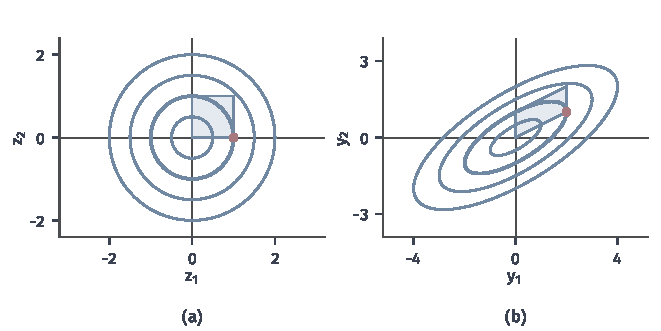
\includegraphics[width=112mm]{figures/07-probability/01-elementary-probability/matplotlib/rvt-linear-gaussian/figure.pdf}
  \caption{线性高斯变换$\bm{Y}=\bm{A}\bm{Z}$，$\bm{A}$的两行为$(2,0)$与$(1,1)$。(a)$\bm{Z}$的等密度线（蓝，圆）与单位正方形（浅蓝），红点为$\bm{z}=(1,0)$。(b)$\bm{Y}$的等密度线（蓝，椭圆）与正方形的像，一个面积为$2$的平行四边形（浅蓝），红点为$\bm{y}=(2,1)$。两幅图的等密度线取同一组$\lVert\bm{z}\rVert_2$值。}
  \label{fig:rvt-linear-gaussian}
\end{BookInlineFigure}

\paragraph{极坐标}
设$X_1,X_2$独立且都服从$\mathcal{N}(0,1)$，问到原点的距离$R$与方向角$\Theta$的分布。映射$(r,\theta)\mapsto(r\cos\theta,r\sin\theta)$把$U=(0,\infty)\times(0,2\pi)$一一地映到平面去掉射线$\{x_1\geq0,\ x_2=0\}$的部分；这条射线面积为零，$(X_1,X_2)$落在上面的概率为零。这里直接把它当作$\bm{h}$，它的Jacobian行列式是
\[
 \det\begin{pmatrix}\cos\theta&-r\sin\theta\\ \sin\theta&r\cos\theta\end{pmatrix}=r .
\]

代入式~\eqref{eq:rvt-multivariate-density}，平方和$x_1^2+x_2^2$变成$r^2$，得到
\begin{equation}
 f_{R,\Theta}(r,\theta)=\frac{1}{2\pi}\mathrm{e}^{-r^2/2}\cdot r=\underbrace{r\,\mathrm{e}^{-r^2/2}}_{R}\cdot\underbrace{\frac{1}{2\pi}}_{\Theta},\qquad r>0,\ 0<\theta<2\pi .
 \label{eq:rvt-polar-density}
\end{equation}
联合密度分解成只含$r$与只含$\theta$的两个因子，所以$R$与$\Theta$独立，$\Theta\sim\operatorname{Unif}(0,2\pi)$，$R$的密度是$r\mathrm{e}^{-r^2/2}$，称为\term{Rayleigh分布}（Rayleigh distribution）。

核对归一化：
\[
 \int_0^\infty r\mathrm{e}^{-r^2/2}\,\mathrm{d}r=\bigl[-\mathrm{e}^{-r^2/2}\bigr]_0^\infty=1 .
\]
由此可算出几个概率：
\[
 \mathbb{P}(R\leq1)=1-\mathrm{e}^{-1/2}\approx0.393,\qquad \mathbb{P}(R>2)=\mathrm{e}^{-2}\approx0.135 .
\]

因子$r$来自面积元。图~\ref{fig:rvt-polar-cell}中，$(r,\theta)$平面上同样大小的小矩形，在$(x_1,x_2)$平面上对应的扇形小块面积约为$r\,\Delta r\,\Delta\theta$，离原点越远越大。所以虽然高斯密度在原点最大，$R$的密度在$r=0$处却是零：靠近原点的圆环面积太小。

\begin{BookInlineFigure}
  \centering
  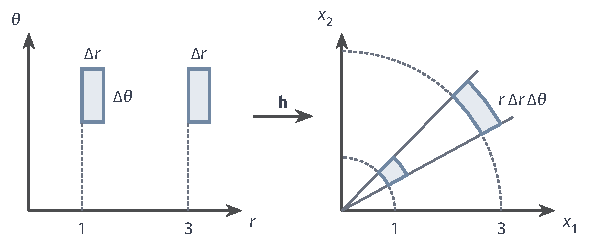
\includegraphics[width=100mm]{figures/07-probability/01-elementary-probability/tikz/rvt-polar-cell/figure.pdf}
  \caption{极坐标的面积元。左侧$(r,\theta)$平面上两个同样大小的矩形（浅蓝），右侧是它们在$(x_1,x_2)$平面上的像，扇形小块的面积约为$r\,\Delta r\,\Delta\theta$，外圈的像比内圈大。}
  \label{fig:rvt-polar-cell}
\end{BookInlineFigure}

再对$W=R^2$用单调变换。$h(w)=\sqrt{w}$，$h'(w)=1/(2\sqrt{w})$，于是
\[
 f_W(w)=\sqrt{w}\,\mathrm{e}^{-w/2}\cdot\frac{1}{2\sqrt{w}}=\frac12\mathrm{e}^{-w/2},\qquad w>0 ,
\]
即$X_1^2+X_2^2\sim\operatorname{Exp}(1/2)$，也就是$\operatorname{Gamma}(1,1/2)=\chi^2_2$。图~\ref{fig:rvt-rayleigh}用模拟样本核对这三个结论。

\begin{BookInlineFigure}
  \centering
  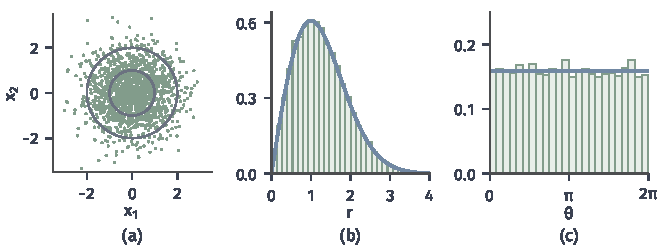
\includegraphics[width=112mm]{figures/07-probability/01-elementary-probability/matplotlib/rvt-rayleigh/figure.pdf}
  \caption{二维标准高斯的极坐标，$20000$个模拟样本（种子$3$）。(a)前$1500$个样本点（绿）与半径$1$、$2$的圆（灰）。(b)$R$的直方图（浅绿）与Rayleigh密度$r\mathrm{e}^{-r^2/2}$（蓝）。(c)$\Theta$的直方图与均匀密度$1/(2\pi)$（蓝）。}
  \label{fig:rvt-rayleigh}
\end{BookInlineFigure}

\paragraph{Gamma归一化}
第~\ref{chap:multivariate-distributions}章用独立Gamma变量除以总和来构造Dirichlet比例，联合密度留到了这里。设$X_1,\ldots,X_d$独立，$X_i\sim\operatorname{Gamma}(\alpha_i,\beta)$，速率$\beta$相同，$d\geq2$。比例$X_i/S$共有$d$个，但它们的和恒为$1$，只有$d-1$个是自由的；只用比例会降维。所以保留总量，取
\[
 S=\sum_{i=1}^{d}X_i,\qquad P_i=\frac{X_i}{S},\quad i=1,\ldots,d-1 ,
\]
这是从$U=(0,\infty)^{d}$到$V=\{(s,\bm{p}):\ s>0,\ p_i>0,\ \sum_{i<d}p_i<1\}$的同维映射。

逆映射是$x_i=sp_i$（$i<d$），$x_d=s(1-p_1-\cdots-p_{d-1})$，所以映射一一。记$p_d=1-\sum_{i<d}p_i$。$\bm{h}$的Jacobian矩阵按列对$s,p_1,\ldots,p_{d-1}$求导，第$i$行（$i<d$）是$(p_i,\ s\bm{e}_i^{\top})$，最后一行是$(p_d,\ -s,\ldots,-s)$。把前$d-1$行都加到最后一行，最后一行变成$(1,0,\ldots,0)$；行列式不变，再按最后一行展开，剩下的子矩阵是$s\bm{I}_{d-1}$，于是
\[
 \bigl\lvert\det D\bm{h}(s,\bm{p})\bigr\rvert=s^{d-1} .
\]

$d=2$时可以直接核对：$x_1=sp$，$x_2=s(1-p)$，行列式是$p\cdot(-s)-s\cdot(1-p)=-s$。

输入的联合密度是各Gamma密度的乘积：
\[
 f_{\bm{X}}(\bm{x})=\prod_{i=1}^{d}\frac{\beta^{\alpha_i}}{\Gamma(\alpha_i)}x_i^{\alpha_i-1}\mathrm{e}^{-\beta x_i}=\frac{\beta^{\alpha_0}\mathrm{e}^{-\beta s}}{\prod_i\Gamma(\alpha_i)}\prod_{i=1}^{d}x_i^{\alpha_i-1},
\]
其中$\alpha_0=\sum_i\alpha_i$，$s=\sum_ix_i$。代入$x_i=sp_i$，乘积变成$s^{\alpha_0-d}\prod_ip_i^{\alpha_i-1}$；再乘以$s^{d-1}$，$s$的幂次是$\alpha_0-1$。按$s$与$\bm{p}$分组，得到
\begin{equation}
 f_{S,\bm{P}}(s,\bm{p})=\underbrace{\frac{\beta^{\alpha_0}}{\Gamma(\alpha_0)}s^{\alpha_0-1}\mathrm{e}^{-\beta s}}_{\operatorname{Gamma}(\alpha_0,\beta)}\cdot\underbrace{\frac{\Gamma(\alpha_0)}{\prod_{i}\Gamma(\alpha_i)}\prod_{i=1}^{d}p_i^{\alpha_i-1}}_{\operatorname{Dir}(\bm{\alpha})} .
 \label{eq:rvt-gamma-dirichlet}
\end{equation}

这一个式子给出四个结论。第一，$S\sim\operatorname{Gamma}(\alpha_0,\beta)$：同速率独立Gamma变量之和仍是Gamma，形状参数相加。第二，比例向量的密度是第二个因子，即$\operatorname{Dir}(\bm{\alpha})$在前$d-1$个自由坐标上的密度。第三，联合密度分解为两个因子，所以总量$S$与比例$\bm{P}$相互独立。第四，$\beta$只出现在第一个因子里，比例的分布与共同速率无关，这就是共同速率被消去的含义。

第二个因子的归一化也随之得到。$f_{S,\bm{P}}$是密度，总积分为$1$；第一个因子对$s$的积分为$1$；所以第二个因子在$V$的$\bm{p}$部分上的积分必为$1$，这就是Dirichlet密度归一化常数的来历。

$d=2$时，比例$P_1=X_1/S$服从$\operatorname{Beta}(\alpha_1,\alpha_2)$。取$\alpha_1=2$、$\alpha_2=3$、$\beta=1$，则$P_1\sim\operatorname{Beta}(2,3)$，均值$2/5$；$S\sim\operatorname{Gamma}(5,1)$，均值$5$。图~\ref{fig:rvt-gamma-simplex}画出两套坐标的对应关系，图~\ref{fig:rvt-dirichlet-check}用模拟核对边缘与独立性。

\begin{BookInlineFigure}
  \centering
  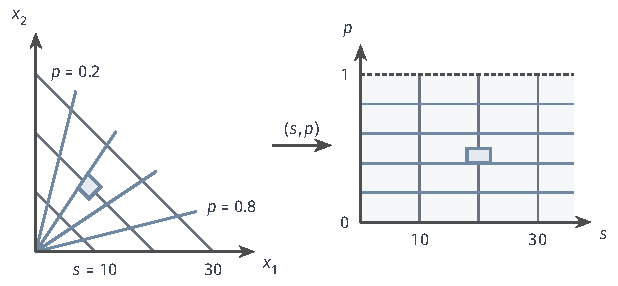
\includegraphics[width=104.7mm]{figures/07-probability/01-elementary-probability/tikz/rvt-gamma-simplex/figure.pdf}
  \caption{总量与比例坐标，$d=2$。左侧第一象限中，灰色斜线是总量$s=x_1+x_2$为常数的线，蓝色射线是比例$p=x_1/s$为常数的线；右侧是对应的$(s,p)$半带。浅蓝小块是$(s,p)$平面上的一个小矩形及其像，像的面积约为$s\,\Delta s\,\Delta p$。}
  \label{fig:rvt-gamma-simplex}
\end{BookInlineFigure}

\begin{BookInlineFigure}
  \centering
  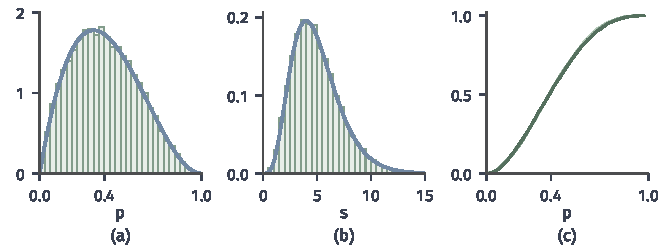
\includegraphics[width=112mm]{figures/07-probability/01-elementary-probability/matplotlib/rvt-dirichlet-check/figure.pdf}
  \caption{Gamma归一化的模拟核对，$X_1\sim\operatorname{Gamma}(2,1)$与$X_2\sim\operatorname{Gamma}(3,1)$独立，$20000$个样本（种子$5$）。(a)$P=X_1/S$的直方图（浅绿）与$\operatorname{Beta}(2,3)$密度（蓝）。(b)$S$的直方图与$\operatorname{Gamma}(5,1)$密度（蓝）。(c)按$S$的三分位数把样本分成三组，三组中$P$的经验分布函数（绿色由浅到深）几乎重合，与$S$独立相符。}
  \label{fig:rvt-dirichlet-check}
\end{BookInlineFigure}

\subsection{多分支与降维}
\label{sec:rvt-branches-reduction}

可逆变换的定理要求同维和一一。两个条件分别失效时，做法与一元时类似：不一一就分支相加，降维就先补足坐标再积掉。

\paragraph{同维多分支}
设$U_1,\ldots,U_m$是互不相交的开集，除去一个面积（体积）为零的集合外覆盖$\bm{X}$的取值范围，$\bm{g}$在每个$U_k$上满足定理~\ref{thm:rvt-multivariate-density}的条件，反函数为$\bm{h}_k$。与定理~\ref{thm:rvt-branch-density}的证明相同，把事件按$\bm{X}$落在哪个$U_k$分解，各分支分别换元再相加，得到
\begin{equation}
 f_{\bm{Y}}(\bm{y})=\sum_{k:\ \bm{y}\in\bm{g}(U_k)}f_{\bm{X}}\bigl(\bm{h}_k(\bm{y})\bigr)\,\bigl\lvert\det D\bm{h}_k(\bm{y})\bigr\rvert .
 \label{eq:rvt-multivariate-branch}
\end{equation}

典型的例子是排序。令$\bm{g}(x_1,x_2)=(\min(x_1,x_2),\max(x_1,x_2))$，输出落在$\{(u,v):\ u<v\}$中。对角线$x_1=x_2$面积为零，去掉之后平面分成$U_1=\{x_1<x_2\}$与$U_2=\{x_1>x_2\}$。在$U_1$上$\bm{g}$是恒等映射，在$U_2$上$\bm{g}$交换两个坐标，两个Jacobian行列式的绝对值都是$1$。于是
\[
 f_{\min,\max}(u,v)=f_{\bm{X}}(u,v)+f_{\bm{X}}(v,u),\qquad u<v .
\]
$X_1,X_2$独立且都服从$\operatorname{Unif}(0,1)$时，结果是三角形$0<u<v<1$上的常数$2$；三角形面积为$1/2$，总积分为$1$。第~\ref{sec:rvt-order-statistics}节把这个计算推广到$n$个变量。

\paragraph{降维映射}
设$Z=X_1+X_2$，映射$\mathbb{R}^2\to\mathbb{R}$。它的导数是$1\times2$的矩阵$(1\ \ 1)$，没有行列式；而且每个$z$的原像是整条直线$\{x_1+x_2=z\}$，不是有限个点，式~\eqref{eq:rvt-multivariate-density}与式~\eqref{eq:rvt-multivariate-branch}都无从套用。

办法是补一个坐标，凑成同维可逆变换。取$W=X_2$，映射$(x_1,x_2)\mapsto(z,w)=(x_1+x_2,x_2)$的逆是$x_1=z-w$、$x_2=w$，Jacobian行列式为$1$。由式~\eqref{eq:rvt-multivariate-density}，
\[
 f_{Z,W}(z,w)=f_{\bm{X}}(z-w,w) .
\]
我们只关心$Z$，把不保留的坐标$w$积掉，就得到边缘密度：
\begin{equation}
 f_Z(z)=\int_{\mathbb{R}}f_{\bm{X}}(z-w,w)\,\mathrm{d}w .
 \label{eq:rvt-sum-completion}
\end{equation}

一般地，若$\bm{Y}=\bm{g}(\bm{X})\in\mathbb{R}^{k}$，$k<d$，且能找到$d-k$个辅助坐标$\bm{W}$使$(\bm{Y},\bm{W})$成为$\bm{X}$的同维可逆变换，就先用式~\eqref{eq:rvt-multivariate-density}求联合密度，再对$\bm{w}$积分。辅助坐标的选法不唯一，只要满足可逆条件，结果都相同；选得好，行列式简单，积分区域也简单。

\paragraph{直接按原像计算}
不便补坐标时，回到分布函数法。仍以$X_1,X_2$独立且都服从$\operatorname{Unif}(0,1)$为例，事件$Z\leq z$的原像是单位正方形中直线$x_1+x_2=z$下方的部分。它的面积分两段计算：
\[
 F_Z(z)=
 \begin{cases}
  z^2/2, & 0\leq z\leq1,\\
  1-(2-z)^2/2, & 1\leq z\leq2 .
 \end{cases}
\]

求导得到三角形密度：$0<z<1$时$f_Z(z)=z$，$1<z<2$时$f_Z(z)=2-z$。用式~\eqref{eq:rvt-sum-completion}也能得到它：被积函数$f_{\bm{X}}(z-w,w)$在$0<w<1$且$0<z-w<1$时为$1$，积分等于这段$w$区间的长度，即$\min(z,2-z)$。

图~\ref{fig:rvt-sum-completion}说明两种做法为什么一致。阈值从$z$增加到$z+\Delta z$时，原像增加了一条斜带，斜带的面积就是$f_Z(z)\Delta z$；式~\eqref{eq:rvt-sum-completion}沿着这条斜带积分，补出的坐标$w$正是斜带上的位置。

\begin{BookInlineFigure}
  \centering
  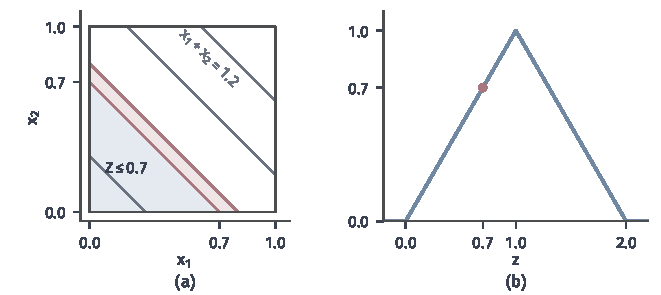
\includegraphics[width=112mm]{figures/07-probability/01-elementary-probability/matplotlib/rvt-sum-completion/figure.pdf}
  \caption{降维映射$Z=X_1+X_2$，$X_1,X_2$独立且服从$\operatorname{Unif}(0,1)$。(a)单位正方形中，浅蓝区域是$Z\leq0.7$的原像，红色斜带是$0.7<Z\leq0.8$的部分，灰线是其他阈值的等值线。(b)$Z$的三角形密度（蓝），红点是$z=0.7$处的值，等于(a)中斜带面积除以$\Delta z=0.1$的极限。}
  \label{fig:rvt-sum-completion}
\end{BookInlineFigure}

其他运算也常这样处理：$\max(X_1,X_2)\leq z$的原像是正方形，$X_1^2+X_2^2\leq z$的原像是圆盘。能写出原像并算出它的概率，就有分布函数；需要密度时再求导。下面四节把这些办法分别用到和、差、乘积、比值和排序上。
